\chapter{Введение}

Конденсатор представляет собой пассивную двухконтактную электрическую пластину, которая хранит потенциальную энергию в электрическом поле. Номинал конденсатора известен как емкость. 

Физическая форма и конструкция практических конденсаторов широко варьируются. Большинство конденсаторов содержат по меньшей мере два электрических проводника часто в виде металлических пластин или поверхностей, разделенных диэлектрической средой. Проводником может быть фольга, тонкая пленка, шарик из металла или электролит. 

Непроводящий диэлектрик действует для увеличения емкости заряда конденсатора. Материалы, используемые в качестве диэлектриков, включают стекло, керамику, пластиковую пленку, бумагу, слюду и оксидные слои. Конденсаторы широко используются как части электрических цепей во многих обычных электрических устройствах. В отличие от резистора идеальный конденсатор не рассеивает энергию.

Когда два проводника испытывают разность потенциалов, например, когда конденсатор прикреплен к батарее, электрическое поле создается через диэлектрик, в результате чего чистый положительный заряд собирается на одной пластине и чистый отрицательный заряд на другой. 

Однако, если на проводах конденсатора подается изменяющееся во времени напряжение, источник проводит постоянный ток из-за циклов зарядки и разрядки конденсатора.

Емкость определяется как отношение электрического заряда на каждом проводнике к разности потенциалов между ними. 

Единицей емкости в Международной системе единиц (СИ) является фарад ($F$), определяемый как один кулон на вольт. Значения емкости типичных конденсаторов для использования в общей электронике колеблются от примерно 1 пикофарада ($pF$) ($10^{-12} F$) до около 1 миллифарада (мФ) ($10^{-3} F$).

Емкость конденсатора пропорциональна площади поверхности пластин (проводников). На практике диэлектрик между пластинами пропускает небольшой ток утечки. Он имеет предел напряженности электрического поля, известный как напряжение пробоя. Проводники приводят к нежелательной индуктивности и сопротивлению.

Конденсаторы широко используются в электронных схемах для блокировки постоянного тока, позволяя проходить переменному току. В сетях аналогового фильтра они сглаживают выход источников питания. В резонансных схемах они настраивают радиостанции на определенные частоты. В системах передачи электроэнергии они стабилизируют поток напряжения и мощности. \cite{ERMUR} Свойство хранения энергии в конденсаторах использовалось как динамическая память на ранних цифровых компьютерах.

\chapter{Работа и комплектующие конденсатора}

Конденсатор состоит из двух проводников, разделенных непроводящей областью \cite{GUSEV}. Непроводящая область может быть либо вакуумной, либо электрическим изоляционным материалом, известным как диэлектрик. Примерами диэлектрических сред являются стекло, воздух, бумага, пластик, керамика и даже область обеднения полупроводников. Из закона Кулона заряд на одном проводнике будет оказывать усилие на носители заряда внутри другого проводника, притягивая заряд противоположной полярности и отталкиваясь от зарядов полярности, поэтому на поверхности другого проводника будет индуцироваться заряд противоположной полярности. Таким образом, проводники имеют равные и противоположные заряды на их обращенных поверхностях \cite{GUSEV}, а диэлектрик развивает электрическое поле.

Идеальный конденсатор характеризуется постоянной емкостью C в фарадах в системе СИ, определяемой как отношение положительного или отрицательного заряда Q на каждом проводнике к напряжению V между ними: \cite{DYAK}

\[
C=\frac{Q}{V}
\]

Емкость одного фарада (F) означает, что один кулон заряда на каждом проводнике вызывает напряжение одного вольта на устройстве. \cite{DYAK} Поскольку проводники (или пластины) находятся близко друг к другу, противоположные заряды на проводниках притягиваются друг к другу из-за их электрических полей, позволяя конденсатору хранить больше заряда для заданного напряжения.

В практических устройствах накопление заряда иногда воздействует на конденсатор механически, вызывая его емкость. 

В этом случае емкость определяется в виде инкрементных изменений:

\[
C=\frac{dQ}{dV}
\]

В гидравлической аналогии носители заряда, протекающие через провод, аналогичны воде, протекающей по трубе. Конденсатор подобен резиновой мембране, запечатанной внутри трубы. Молекулы воды не могут проходить через мембрану, но некоторая жидкость может двигаться, растягивая мембрану. 

Аналогия поясняется несколькоми аспектами конденсаторов:

\begin{itemize}
	\item Ток изменяет заряд на конденсаторе, так же как поток воды изменяет положение мембраны. В частности, эффект электрического тока заключается в увеличении заряда одной пластины конденсатора и уменьшении заряда другой пластины на равное количество. Это происходит так же, как когда поток воды перемещает резиновую мембрану, он увеличивает количество воды на одной стороне мембраны и уменьшает количество воды с другой стороны.
	\item Чем больше заряжается конденсатор, тем больше его падение напряжения; то есть чем больше он «отталкивается» от зарядного тока. Это аналогично более растянутой мембране, тем более она отталкивает воду.
	\item Заряд может протекать «через» конденсатор, даже если никакой отдельный электрон не может попасть с одной стороны на другую. Это аналогично воде, протекающей по трубе, хотя молекула воды не проходит через резиновую мембрану. Поток не может продолжаться в одном направлении всегда; конденсатор испытывает диэлектрический пробой, и аналогично мембрана в конечном итоге разорвется.
	\item Емкость описывает, сколько заряда может храниться на одной пластине конденсатора при заданном «нажатии» (падение напряжения). Очень эластичная гибкая мембрана соответствует более высокой емкости, чем жесткая мембрана.
\end{itemize}


\chapter{Цепи переменного тока}

Импеданс, векторная сумма реактивности и сопротивления, описывает разность фаз и отношение амплитуд между синусоидально изменяющимся напряжением и синусоидально изменяющимся током на заданной частоте. Анализ Фурье позволяет построить любой сигнал из спектра частот, откуда можно найти реакцию схемы на различные частоты. Реактивное сопротивление и импеданс конденсатора соответственно

\[
X = - \frac{1}{\omega C} = - \frac{1}{2 \pi f  C}; 
Z = \frac{1}{j \omega C}
\]

где $j$ - мнимая единица, а $\omega$ - угловая частота синусоидального сигнала. Фаза $-j$ указывает, что переменное напряжение $U = ZI$ отстаёт от переменного тока на $90\deg $: фаза положительного тока соответствует увеличению напряжения при заряде конденсатора; нулевой ток соответствует мгновенному постоянному напряжению и т. д.

Импеданс уменьшается с увеличением емкости и увеличением частоты. Это означает, что высокочастотный сигнал или более большой конденсатор приводят к более низкой амплитуде напряжения на амплитуду. 

Конденсаторы отличаются от резисторов и индукторов тем, что импеданс обратно пропорционален определяющей характеристике.

\chapter{Типы конденсаторов}
Практические конденсаторы доступны в коммерческих целях в самых разных формах. Тип внутреннего диэлектрика, структура пластин и упаковка устройства сильно влияют на характеристики конденсатора и его применения.

Доступные значения варьируются от очень низкого (диапазон пикофарада, в то время как в принципе возможны сколь угодно низкие значения) до 5 кФ суперконденсаторов.

Выше примерно 1 микрофарад электролитические конденсаторы обычно используются из-за их небольшого размера и низкой стоимости по сравнению с другими типами.

Высококонцентрированные суперконденсаторы используют пористый материал на основе углеродного электрода.

\chapter{Диэлектрические материалы}

Большинство конденсаторов имеют диэлектрическую прокладку, которая увеличивает их емкость по сравнению с воздухом или вакуумом. Чтобы максимизировать заряд, который может удерживать конденсатор, диэлектрический материал должен иметь как можно большую диэлектрическую проницаемость, а также иметь как можно больше напряжение пробоя. Диэлектрик также должен иметь как можно меньшую потерю с частотой, насколько это возможно.

Тем не менее, конденсаторы с низким значением доступны с вакуумом между их пластинами, чтобы обеспечить чрезвычайно высокое напряжение и низкие потери. 

В последующих конструкциях используется полимерная фольга из диэлектриков между подвижными и неподвижными пластинами, без значительного воздушного пространства между пластинами.

Доступны несколько твердых диэлектриков, включая бумагу, пластик, стекло, слюду и керамику. Бумага широко использовалась в старых конденсаторах и обеспечивает относительно высокую производительность. Однако бумага поглощает влагу и в значительной степени заменяется пластиковыми пленочными конденсаторами.

Большинство используемых ныне пластиковых пленок обеспечивают лучшую стабильность и эффективность старения, чем такие старые диэлектрики, как масляная бумага, что делает их полезными в таймерных цепях, хотя они могут быть ограничены относительно низкими рабочими температурами и частотами из-за ограничений пластика используемая пленка. Большие конденсаторы пластиковой пленки широко используются в цепях подавления, схемах запуска двигателя и схемах коррекции коэффициента мощности.

Керамические конденсаторы, как правило, небольшие, дешевы и полезны для высокочастотных применений, хотя их емкость сильно зависит от напряжения и температуры, и они плохо развиваются. Они также могут страдать от пьезоэлектрического эффекта. Керамические конденсаторы широко классифицируются как диэлектрики класса 1, которые имеют предсказуемое изменение емкости с температурой или диэлектриком класса 2, которые могут работать при более высоком напряжении. Современная многослойная керамика, как правило, довольно мала, но некоторые типы имеют по своей сути широкие допуски по стоимости, микрофонические проблемы и обычно физически хрупкие.

Конденсаторы из стекла и слюды чрезвычайно надежны, стабильны и устойчивы к высоким температурам и напряжениям, но слишком дороги для большинства основных применений.

Электролитические конденсаторы и суперконденсаторы используются для хранения малых и больших количеств энергии, соответственно, керамические конденсаторы часто используются в резонаторах, а паразитная емкость возникает в схемах, где простая структура проводника-диэлектрика-проводника формируется непреднамеренно по конфигурации схемы

\begin{figure}[h!]
	\centering
	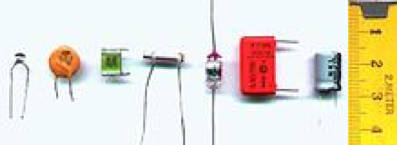
\includegraphics[width=.4\textwidth]{images/1.png}
\end{figure}

Считая с левой стороны: многослойная керамика, керамический диск, многослойная полиэфирная пленка, трубчатая керамика, полистирол, металлизированная полиэфирная пленка, алюминиевый электролиз. Деления крупных масштабов находятся в сантиметрах.

Электролитические конденсаторы используют алюминиевую или танталовую пластину с оксидным диэлектрическим слоем. 

Второй электрод представляет собой жидкий электролит, соединенный с контуром другой фольгой. Электролитические конденсаторы обладают очень высокой емкостью, но имеют слабые допуски, высокую нестабильность, постепенную потерю емкости, особенно при нагревании, и высокий ток утечки. В некачественных конденсаторах может течь электролит, что вредно для печатных плат. Проводимость электролита падает при низких температурах, что увеличивает эквивалентное последовательное сопротивление. Несмотря на то, что они широко используются для кондиционирования питания, плохие высокочастотные характеристики делают их непригодными для многих применений. Электролитические конденсаторы страдают от самодеградации, если они не используются в течение периода (около года). Например, в более старом оборудовании это может вызвать образование дуги в трубах выпрямителя. Их можно восстановить перед использованием, постепенно применяя рабочее напряжение, часто выполняемое на старинном вакуумном трубном оборудовании в течение тридцати минут, используя переменный трансформатор для питания переменного тока. Использование этого метода может быть менее удовлетворительным для некоторых твердотельных устройств, которые могут быть повреждены при работе ниже нормального диапазона мощности, требуя, чтобы источник питания сначала был изолирован от потребляющих контуров. Такие средства защиты могут быть неприменимы к современным высокочастотным источникам питания, поскольку они обеспечивают полное выходное напряжение даже при уменьшенном входном напряжении. 

Конденсаторы тантала обеспечивают лучшие характеристики частоты и температуры, чем алюминий, но более высокое поглощение и утечка диэлектрика. \cite{ERMUR}



\chapter{Заключение}

Конденсатор — двухполюсник с постоянным или переменным значением емкости малой проводимостью; устройство для накопления заряда и энергии электрического поля.

Конденсатор является пассивным электронным компонентом. В простейшем варианте конструкция состоит из двух электродов в форме пластин (называемых обкладками), разделённых диэлектриком, толщина которого мала по сравнению с размерами обкладок (см. рис.). Практически применяемые конденсаторы имеют много слоёв диэлектрика и многослойные электроды, или ленты чередующихся диэлектрика и электродов, свёрнутые в цилиндр или параллелепипед со скруглёнными четырьмя рёбрами (из-за намотки). Ёмкость конденсатора измеряется в фарадах.
